% grupos de hablantes viejo
% la primer entrega de cross validation 

\subsection{Grupos de hablantes}

%Para medir el rendimiento de los distintos clasificadores definimos un modelo de testing. Este separa una parte de los datos obtenidos para entrenar el clasificador y otro para testearlo.

La complejidad del problema y la forma en que fue realizado el experimento nos lleva a tener que descartar un modelo de testing común. Si utilizamos un modelo estándar deberíamos dividir los audios en dos grupos, uno lo usaríamos para entrenar y otro para testear. En este contexto, podría surgir el problema de que un hablante tenga audios en el conjunto de train y también en el de test. En ese caso el test sería erróneo ya que podría suceder que estaríamos entrenando con audios de un hablante que luego sería testeado en otro audio.

Para evitar este inconveniente debimos tomar en cuenta los hablantes a la hora de dividir los grupos. Dividimos \textbf{a los hablantes} en dos conjuntos: uno llamado train que se utiliza para entrenar, y otro test que testea el clasificador entrenado. Si bien esto evita el problema anterior, la cantidad de audios aportados por cada hablante fue muy variable: viendo el conjunto de datos, el hablante que aportó más grabaciones realizó 30 de las mismas, mientras que el hablante que aportó menos realizó 1 solamente. Tomando en cuenta esto, la cantidad de audios de un conjunto puede quedar muy desbalanceada con respecto al otro. Por ejemplo, puede pasar que la cantidad de audios en test sea mayor a la de train. Este caso lo queremos descartar ya que estaríamos intentando clasificar sin haber entrenado lo suficiente. Para mitigar este problema, hicimos que el conjunto de train tenga el 70\% de las instancias mientras que el restante 30\% sea destinado para test. Estos dos grupos conformaron un par que lo llamaremos \textit{fold}. Asegurándonos que tenemos más instancias en train que en test evitamos tener folds con pocas instancias para entrenar.

\begin{figure}[H]
	\begin{tikzpicture}[node distance=1cm]
	
	\node (train1) [train] {Train};
	\node (train2) [train, xshift=-3.0cm] {Train};
	\node (train3) [train, xshift=-6.0cm] {Train};
	\node (train4) [train, xshift=-9.0cm] {Train};
	\node (train5) [train, xshift=-12.0cm] {Train};
	
	\node (data) [datos, below of=train5, yshift=4.0cm,  xshift=6.0cm] {Datos};
	
	\node (fold1) [fold, above of=train5] {\textit{Fold 1}};
	\node (fold2) [fold, above of=train4] {\textit{Fold 2}};
	\node (fold3) [fold, above of=train3] {\textit{Fold 3}};
	\node (fold4) [fold, above of=train2] {\textit{Fold 4}};
	\node (fold5) [fold, above of=train1] {\textit{Fold 5}};
	
	\node (test1) [test, below of=train1] {Test};
	\node (test2) [test, below of=train2] {Test};
	\node (test3) [test, below of=train3] {Test};
	\node (test4) [test, below of=train4] {Test};
	\node (test5) [test, below of=train5] {Test};
	
	\node (proc1) [proc, below of=test1, yshift=-1.2cm] {Entrenar y testear};
	\node (proc2) [proc, below of=test2, yshift=-1.2cm] {Entrenar y testear};
	\node (proc3) [proc, below of=test3, yshift=-1.2cm] {Entrenar y testear};
	\node (proc4) [proc, below of=test4, yshift=-1.2cm] {Entrenar y testear};
	\node (proc5) [proc, below of=test5, yshift=-1.2cm] {Entrenar y testear};
	
	\node (prom) [prom, below of=test3, yshift=-3.0cm] {Promedio};
	
	\draw [arrowBig] (data) -- (fold3);
	
	\draw [arrow] (test1) -- (proc1);
	\draw [arrow] (test2) -- (proc2);
	\draw [arrow] (test3) -- (proc3);
	\draw [arrow] (test4) -- (proc4);
	\draw [arrow] (test5) -- (proc5);
	
	\draw [arrow] (proc1) -- (prom);
	\draw [arrow] (proc2) -- (prom);
	\draw [arrow] (proc3) -- (prom);
	\draw [arrow] (proc4) -- (prom);
	\draw [arrow] (proc5) -- (prom);
	
	\end{tikzpicture}
	\caption{Esquema de test 5-folds}
	\label{graficoFold}
\end{figure}


No podemos quedarnos con un solo fold, ya que podría encasillar el resultado para \textit{ese} conjunto en particular. Es por esto que creamos 5 folds de la forma $<$train, test$>$ con las características antes descriptas. Este modelo de testing se denomina \textbf{cross-validation test de 5-folds}. El promedio de los porcentajes de instancias correctas de cada fold va a darnos la performance total. De esta forma, el resultado es independiente de la partición de los datos de entrenamiento y prueba. En la Figura \ref{graficoFold} se diagrama este modelo de testing.


Otro problema a tener en cuenta es que los grupos de test generados sean lo más distintos posibles. Este requerimiento no es tan sencillo si uno posee tan pocas instancias, ya que podría suceder que se repita mucha cantidad de instancias entre folds haciendo que no sea provechoso el test. Para solucionar esto, el test de cross-validation fue realizado de la siguiente forma: armamos conjuntos a partir de las instancias para train y test, pero con una salvedad. Para armar el conjunto de test utilizamos el 20\% de los elementos de las instancias ya utilizadas en los tests anteriores y el resto de instancias nuevas. De esta forma, regulamos la cantidad de instancias repetidas en los tests y nos aseguramos que sean todos distintos. Esto nos permitió utilizar instancias nuevas en los 5 folds. 

%A continuación el código generador del test cross-validation:
%\lstset{ %
%	language=C++,                % choose the language of the code
%	basicstyle=\footnotesize,       % the size of the fonts that are used for the code
%	numbers=left,                   % where to put the line-numbers
%	numberstyle=\small,      % the size of the fonts that are used for the line-numbers
%	stepnumber=1,                   % the step between two line-numbers. If it is 1 each line will be numbered
%	numbersep=1pt,                  % how far the line-numbers are from the code
%	backgroundcolor=\color{white},  % choose the background color. You must add \usepackage{color}
%	showspaces=false,               % show spaces adding particular underscores
%	showstringspaces=false,         % underline spaces within strings
%	showtabs=false,                 % show tabs within strings adding particular underscores
%	frame=lines,           % adds a frame around the code
%	tabsize=1,          % sets default tabsize to 2 spaces
%	captionpos=b,           % sets the caption-position to bottom
%	breaklines=true,        % sets automatic line breaking
%	postbreak=\raisebox{0ex}[0ex][0ex]{\ensuremath{\hookrightarrow\space}},
%	breakatwhitespace=false,    % sets if automatic breaks should only happen at whitespace
%	escapeinside={\%*}{*)},          % if you want to add a comment within your code
%	morekeywords={GeneradorDeTest, porcentajeMaximoDeSimilitud, checkBalance, Input, Output, Repetir, veces, Si, Agregar, Recorrer, Devolver, y, no, esta, en},
%	literate= {<-} {$\le$}{2} {!=} {$\neq$}{2} {<-} {$\leftarrow$}{2} {==} {=}{2} {&&} {$\cap$}{2} {||} {$\cup$}{2} }
%\begin{lstlisting}
%GeneradorDeTest:
%      Input: conjunto audios
%      Output: conjunto de <train, test>
%      resultado <-{}
%      train <- {}
%      test <- {}
%      hablantesEnTest <- {}
%      hablantes <- ObtenerHablantes(audios)
%      tamTest <- tam(hablantes) * 0.3 
%      #Esta cte nos define el tamano del fold
%      
%      Repetir 5 veces:
%      {
%      hablantesUsadosEnTest <- ElegirRandom(hablantesEnTest, tamTest * 0.2) 
%      #Esta cte nos define porcentaje de hablantes usados
%
%      hablantesNoUsadosEnTest <- ElergirRandom(hablantes - hablantesEnTest, tamTest * 0.8) #Idem hablantes nuevos
%
%      hablantesTest <- hablantesEnTest + hablantesNoUsadosEnTest
%
%      test <- ObtenerAudios(hablantesTest, audios)
%      train <- ObtenerAudios(hablantes - hablantesTest, audios)
%
%      Si <train, test> no est'a en resultado #No es un fold ya creado
%      y porcentajeMaximoDeSimilitud(test, resultado, 0.2) 
%      #El test creado solo puede ser 20 % parecido a uno anterior
%      y checkBalance(train) y checkBalance(test) 
%      #Chequeo del balance entre audios de BsAs y Cba
%            {
%                  Agregar <train, test> a resultado
%                  Agregar hablantesTest a hablantesEnTests
%            }
%      }
%      Devolver resultado
%
%porcentajeMaximoDeSimilitud:
%      Input: conj, conjunto de fold, pctMax
%      Output: booleano
%      Recorrer test de conjunto de fold:
%      {
%            pct <- Maximo(pct, porcentajeSimilitud(conj, test))
%      }
%      Devolver pct < pctMax
%
%checkBalance:
%      Input: conj
%      Output: booleano
%      ck_bsas <- #(conj) * 0.50 < #bsas(conj) < #(conj) * 0.70
%      ck_cba <- #(conj) * 0.25 < #cba(conj) < #(conj) * 0.45
%      ck_both <- #cba(conj) < #bsas(conj)
%      Devolver ck_bsas y ck_cba y ck_both
%\end{lstlisting}
%
%El algoritmo principal itera 5 veces para crear cada fold. En cada iteración, elige el 80\% de hablantes anteriormente no usados en ningún test y el 20\% restante de hablantes anteriormente ya usados. La elección de cada uno se realiza de forma azarosa. Esto se puede ver en las líneas 13 y 16. Luego, se obtienen de cada uno de los hablantes sus respectivos audios (líneas 19 y 20). Finalmente se chequea que el fold generado cumpla con las restricciones que habíamos definido. Estas son: el fold generado no se creó anteriormente, el test sólo tiene como máximo 20\% de elementos repetidos de los demás tests (líneas 20 y 26) y que las cantidades de audios de Córdoba y de Buenos Aires están balanceadas.
%
%La función $porcentajeMaximoDeSimilitud$ nos permite chequear que el conjunto de test generado en una iteración en particular tiene a lo sumo 20\% de audios en común con las demás instancias.
%
%La función $checkBalance$ determina si un conjunto cumple con las restricciones de balance. La primer restricción corresponde a que el porcentaje de audios de Buenos Aires en este conjunto debe ser entre 50-70\%. La segunda restricción corresponde al porcentaje de Córdoba y debe ser entre 25-45\%. Estos porcentajes intentan balancear cada test evitando que un sólo test acapare todas las instancias posibles a testear. Finalmente, la última condición pide tener más audios de Buenos Aires que de Córdoba para no agotar las instancias cordobesas.

\subsubsection{Resultados}

Recordemos que al tener pocos datos debimos repetir instancias en los grupos de tests. El porcentaje de instancias repetidas es menor al 20\%. Vamos a mostrar como son estos conjuntos:

\begin{figure}[H]
	\centering
	\pgfplotsset{width=10cm, height=6cm}
	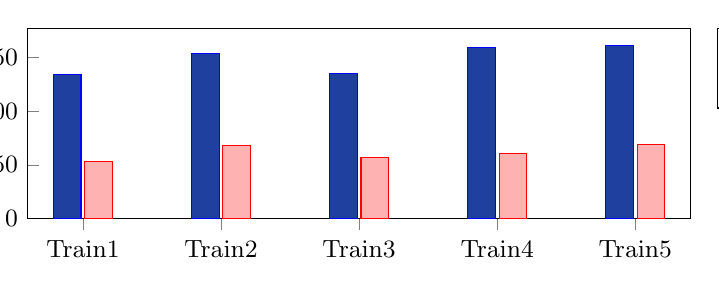
\begin{tikzpicture}[trim axis left, trim axis right]
	\begin{axis}[
	ybar,
	area legend,
	tick label style={font=\small},
	tickpos=left,
	xticklabels={Train1, Train2, Train3, Train4, Train5}, 
	xtick={1,2,3,4,5},
	ymin=0,
	legend entries={BsAs,Cba},
	legend style={at={(1.04,1.002)}, anchor=north west,draw=black}, 
	]
	\addplot +[bar shift=-.2cm, area legend, fill={rgb:red,1;green,2;blue,5}] coordinates {(1,134) (2,154) (3,135) (4,159) (5,161)};
	
	\addplot  +[bar shift=.2cm, area legend]coordinates {(1,53) (2,68) (3,57) (4,61) (5,69)};
	\end{axis}
	\end{tikzpicture}
\end{figure}

\begin{figure}[H]
	\centering
	\pgfplotsset{width=10cm, height=4cm}
	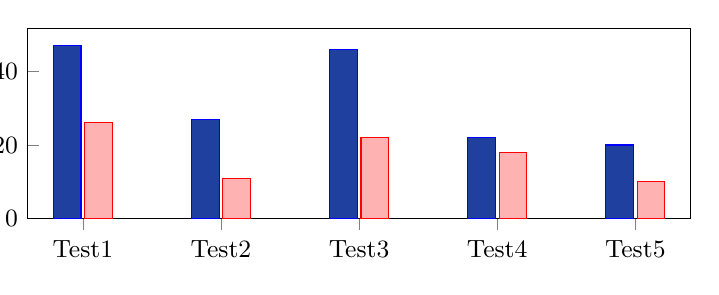
\begin{tikzpicture}[trim axis left, trim axis right]
	\begin{axis}[
	ybar,
	tick label style={font=\small},
	tickpos=left,
	xticklabels={Test1, Test2, Test3, Test4, Test5}, 
	xtick={1,2,3,4,5},
	ymin=0,
	]
	\addplot +[bar shift=-.2cm, area legend, fill={rgb:red,1;green,2;blue,5}] coordinates {(1,47) (2,27) (3,46) (4,22) (5,20)};
	
	\addplot  +[bar shift=.2cm, area legend]coordinates {(1,26) (2,11) (3,22) (4,18) (5,10)};
	\end{axis}
	\end{tikzpicture}
	\caption{Cantidad de instancias de Buenos Aires y Córdoba según cada grupo de Train y Tests}
	\label{TestsInstances}
\end{figure}

La tabla \ref{class_corr_en_pct} resume los resultados de clasificación correcta (en porcentaje) para los distintos clasificadores.

\begin{table}[H]
	\centering
	\begin{tabular}{|l|c|c|c|c|c|c|}
		\hline
		\textbf{}  & \textbf{Zero Rule} & \textbf{Ripper} & \textbf{C4.5} & \textbf{SVM} & \textbf{NaiveBayes} \\ \hline
		\textbf{Fold 1}  & 64 & 61 & 64 & 73 & 63 \\ \hline
		\textbf{Fold 2}  & 71 & 68 & 71 & 76 & 71 \\ \hline
		\textbf{Fold 3}  & 67 & 54 & 45 & 75 & 67 \\ \hline
		\textbf{Fold 4}  & 55 & 52 & 55 & 67 & 80 \\ \hline
		\textbf{Fold 5}  & 66 & 70 & 66 & 70 & 70 \\ \hline
		\hline \hline
		\textbf{Promedio} & 64 & 61 & 60 & 72 & 70 \\ \hline
	\end{tabular}
	\caption{Clasificación correcta en porcentaje}
	\label{class_corr_en_pct}
\end{table}

En esta tabla, Fold 1 corresponde al primer par $<$train, test$>$, Fold 2 al segundo par y así sucesivamente. En la Figura \ref{porcentajexClasificador} se puede ver gráficamente los resultados de clasificación correcta de dicha tabla. Excluimos a Ripper y C4.5 por dar muy parecido a Zero Rule.

\begin{figure}[H]
	\centering
	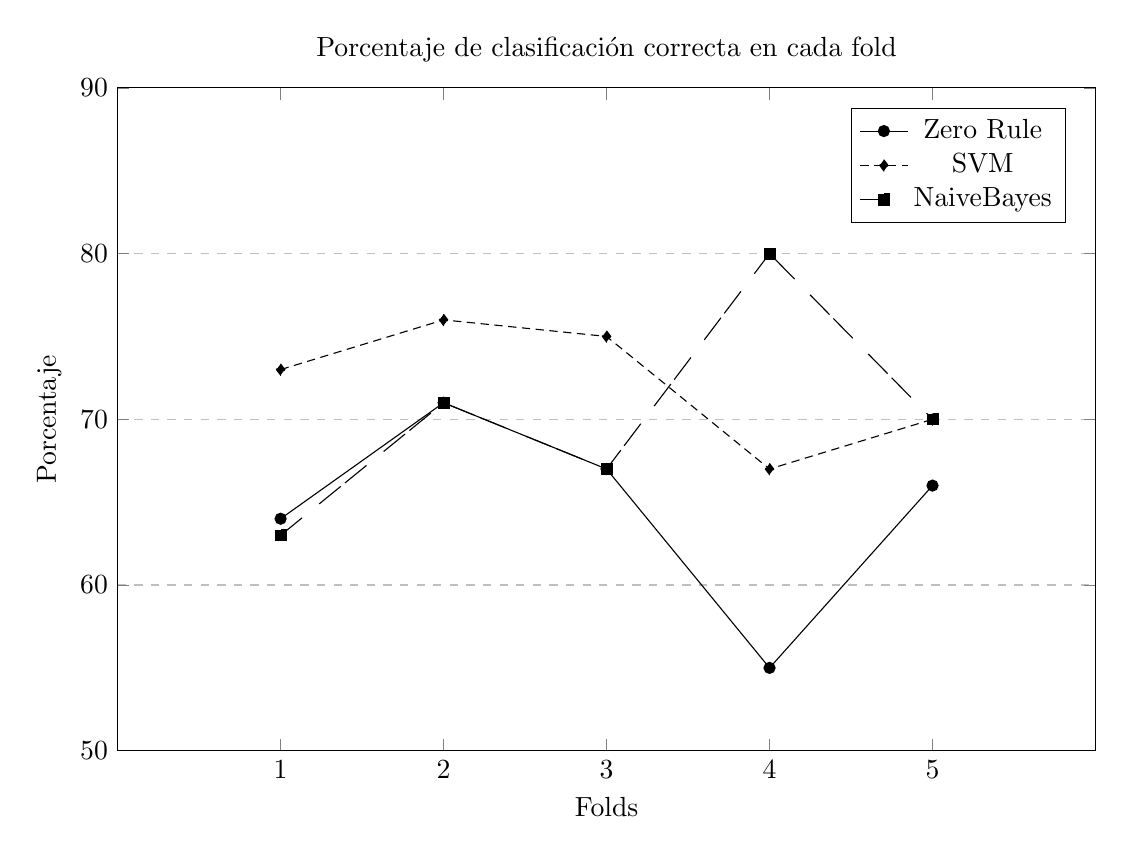
\begin{tikzpicture}
	\begin{axis}[
	width=14cm,
	height=10cm,
	title={Porcentaje de clasificación correcta en cada fold},
	xlabel={Folds},
	ylabel={Porcentaje},
	xmin=0, xmax=6,
	ymin=50, ymax=90,
	xtick={1,2,3,4,5},
	ytick={20,30,40,50,60,70,80,90,100},
	legend pos=north east,
	ymajorgrids=true,
	grid style=dashed
	] 
	\addplot [mark=otimes*, width=1pt] coordinates {
		(1,64)(2,71)(3,67)(4,55)(5,66) };\addlegendentry{Zero Rule};
	%\addplot[mark=diamond*,dash pattern=on 10pt off 2pt on 3pt off 2pt]coordinates {
	%    (1,61)(2,68)(3,54)(4,52)(5,70) };\addlegendentry{JRip};
	\addplot [mark=diamond*,dash pattern=on 3pt off 2pt on 3pt off 2pt]coordinates {
		(1,73)(2,76)(3,75)(4,67)(5,70) };\addlegendentry{SVM};
	\addplot [mark=square*,dash pattern=on 10pt off 8pt on 10pt off 2pt]coordinates {
		(1,63)(2,71)(3,67)(4,80)(5,70) };\addlegendentry{NaiveBayes};
	\end{axis}
	\end{tikzpicture}
	\caption{Porcentaje de Zero Rule, SVM y NaiveBayes}
	\label{porcentajexClasificador}
\end{figure}

Recordemos que el clasificador Zero Rule elige siempre la clase mayoritaria en su grupo de test. Viendo la Figura \ref{porcentajexClasificador} podemos notar que Zero Rule mantiene un porcentaje en los diferentes tests entre un 55\% y casi 70\%. El clasificador Support vector machine (SVM) siempre se mantiene por arriba de este Baseline.

Algo interesante sucede con el clasificador NaiveBayes: muestra resultados muy similares a Zero Rule pero en el test 4 posee mucha mejor performance. Viendo los grupos generados en la Figura \ref{TestsInstances}, el fold 4 es el que tiene menos diferencia entre cantidad de hablantes de Buenos Aires y Córdoba. Al tener mitad instancias de cada grupo y como Zero Rule elige entre uno de esos dos, va a poseer un porcentaje de acierto cercano al 50\%, como sucede.  

El porcentaje de exactitud en la clasificación se puede apreciar con las métricas \textit{Precision} y \textit{Recall}. \textit{Precision} se define como la cantidad de verdaderos positivos sobre la cantidad de verdaderos y falsos positivos. \textit{Recall} se define como la cantidad de verdaderos positivos sobre la cantidad de verdaderos positivos y falsos negativos. Tomamos como verdaderos positivos a la condición de que fue clasificado como Buenos Aires y efectivamente es de ahí. Falsos negativos si el hablante es de Buenos Aires pero es clasificado como Córdoba. Y falso positivo si el hablante es de Córdoba pero es clasificado como Buenos Aires. 

%http://en.wikipedia.org/wiki/Precision_and_recall

Las Figuras \ref{ZeroR_matrizconf}, \ref{FSMO_matrizconf} y \ref{NaiveBayes_matrizconf} muestran los valores que  surgen de la matriz de confusión. Vamos a analizar como son estas métricas para el caso del test 4, que es el más interesante.

% Precision = VP / VP + FP
% Recall = VP / VP + FN
% VP = "BsAs classif. como BsAs"
% FN = "BsAs classif. como Cba"
% FP = "Cba classif. como BsAs" 

%\begin{center}
%\Large Matrices de confusión para test 4
%\end{center}

\begin{figure}[H]
	\centering
	\paragraph*{Zero Rule:}\mbox{}\\
	\begin{table}[H]
		\centering
		\begin{tabular}{|c|c|l|c|c|c|c|}
			\hline
			BsAs & Cba &  \\ \hline
			22 &  18 &  Clasificado como BsAs \\ \hline
			0  &   0 &  Clasificado como Cba \\ \hline
		\end{tabular}
	\end{table}
	\begin{center}
		\textbf{Precision = 22/40 = 0.55;} \textbf{Recall = 1}\\
		\textbf{Instancias correctas = 55\%}
	\end{center}
	\caption{Matriz de confusión para Zero Rule en el test 4}
	\label{ZeroR_matrizconf}
\end{figure}

\begin{figure}[H]
	\centering
	\paragraph*{Support vector machine:}\mbox{}\\
	\begin{table}[H]
		\centering
		\begin{tabular}{|c|c|l|c|c|c|c|}
			\hline
			BsAs & Cba &  \\ \hline
			22 &  13 &  Clasificado como BsAs \\ \hline
			0  &   5 &  Clasificado como Cba \\ \hline
		\end{tabular}
	\end{table}
	\begin{center}
		\textbf{Precision = 22/35 = 0.63;} \textbf{Recall = 1}\\
		\textbf{Instancias correctas = 67\%}
	\end{center}
	\caption{Matriz de confusión para SVM en el test 4}
	\label{FSMO_matrizconf}
\end{figure}

\begin{figure}[H]
	\centering
	\paragraph*{NaiveBayes:}\mbox{}\\
	\begin{table}[H]
		\centering
		\begin{tabular}{|c|c|l|c|c|c|c|}
			\hline
			BsAs & Cba &  \\ \hline
			20 &  6 &  Clasificado como BsAs \\ \hline
			2  &  12 &  Clasificado como Cba \\ \hline
		\end{tabular}
	\end{table}
	\begin{center}
		\textbf{Precision = 20/26 = 0.77;} \textbf{Recall = 20/22 = 0.9}\\
		\textbf{Instancias correctas = 80\%}
	\end{center}
	\caption{Matriz de confusión para NaiveBayes en el test 4}
	\label{NaiveBayes_matrizconf}
\end{figure}

Viendo estas matrices de confusión y sus métricas podemos observar cuál es el error que se produce en cada uno de los clasificadores. Notamos que Zero Rule produce mucho \textit{Error de tipo I} (clasificador afirma que es de Buenos Aires y en realidad es de Córdoba). Esto sucede ya que elige sólo una categoría siempre. En los demás clasificadores se intenta realmente predecir y por eso los Errores de tipo I y II están más distribuidos.

Otro dato a tener en cuenta es que, si bien el clasificador Zero Rule tuvo un valor alto en la métrica \textit{Recall}, no fue lo mismo para \textit{Precision} y por eso el valor de instancias correctas dio bastante malo. Ambos valores deben estar cercanos al 1 para tener una buena performance. Por eso en el caso de NaiveBayes; si bien ningún valor dio 1, ambos están cerca y posee en mayor porcentaje de instancias correctas.

Puede suceder que el porcentaje de instancias correctas sea el mismo pero los Errores de tipo I y II sean más balanceados. Esto es el caso del conjunto de test 1. Las tablas de las Figuras \ref{ZeroR_matrizconf_2}, \ref{NaiveBayes_matrizconf_2} muestran este caso para los clasificadores Zero Rule y NaiveBayes.

%\begin{center}
%\Large Matrices de confusión para test 1
%\end{center}

\begin{figure}[H]
	\centering
	\paragraph*{Zero Rule:}\mbox{}\\
	\begin{table}[H]
		\centering
		\begin{tabular}{|c|c|l|c|c|c|c|}
			\hline
			BsAs & Cba &  \\ \hline
			47 &  26 &  Clasificado como BsAs \\ \hline
			0 &  0 &  Clasificado como Cba \\ \hline
		\end{tabular}
	\end{table}
	\begin{center}
		\textbf{Precision = 47/73 = 0.64;} \textbf{Recall = 47/47 = 1}\\
		\textbf{Instancias correctas = 64\%}
	\end{center}
	\caption{Matriz de confusión para Zero Rule en el test 1}
	\label{ZeroR_matrizconf_2}
\end{figure}

\begin{figure}[H]
	\centering
	\paragraph*{NaiveBayes:}\mbox{}\\
	\begin{table}[H]
		\centering
		\begin{tabular}{|c|c|l|c|c|c|c|}
			\hline
			BsAs & Cba &  \\ \hline
			33 &  13 &  Clasificado como BsAs \\ \hline
			14 &  13 &  Clasificado como Cba \\ \hline
		\end{tabular}
	\end{table}
	\begin{center}
		\textbf{Precision = 33/46 = 0.7;} \textbf{Recall = 33/47 = 0.7}\\
		\textbf{Instancias correctas = 63\%}
	\end{center}
	\caption{Matriz de confusión para NavieBayes en el test 1}
	\label{NaiveBayes_matrizconf_2}
\end{figure}

En este caso notamos que, a pesar de que el porcentaje de instancias correctas den valores cercanos, Zero Rule concentra gran parte del error en un tipo sólo, mientras que NaiveBayes lo distribuye entre los dos tipos.

No realizaremos los tests estadísticos de Wilcoxon y Test t de Student para este modelo de test. La razón es que los conjuntos de test de cada fold no son independientes. Recordemos que tienen 20 \% de instancias repetidas, entonces cada fold por separado no es estadísticamente independiente. Es por ello que dejamos de lado los tests estadísticos.

%\subsection{Wilcoxon y Test t de Student}
%
%En esta sección mostramos los resultados de estos tests estadísticos. Recordemos que los resultados surgieron de realizar los test de Wilcoxon y t de Student para el vector resultado de cada clasificador con respecto a ZeroR. Los resultados expresados en p-valor se pueden observar en la tabla \ref{res_tests_wilcoxon_student}.
%
%\begin{table}[H]
%	\centering
%	\begin{tabular}{|l|c|c|c|c|c|c|}
%		\hline
%		\textbf{}  & \textbf{Student Test} & \textbf{Wilcoxon Test} \\ \hline
%		\textbf{ZeroR y JRip}  & 0.8438 & 0.87 \\ \hline
%		\textbf{ZeroR y J48}  & 0.9772 & 0.813 \\ \hline
%		\textbf{ZeroR y NaiveBayes}  & 0.2113 & 0.1692 \\ \hline
%		\textbf{ZeroR y Function SMO}  & 0.03125 & 0.004545 \\ \hline
%	\end{tabular}
%	\caption{Resultados de cada test representado en p-valor}
%	\label{res_tests_wilcoxon_student}
%\end{table}
%
%Todos los clasificadores pasaron el test Shapiro-Wilk, entonces podemos afirmar que los resultados de cada clasificador corresponden a una distribución Normal. Analizando los resultados resumidos en la Figura \ref{res_tests_wilcoxon_student} notamos que para el clasificador Function SMO posee p-valor menor a 0,05 en ambas columnas. Esto quiere decir que para \textbf{Function SMO hay evidencia suficiente de ser mejor que ZeroR}. Por otro lado, los demás no pudieron lograr este cometido. 

\subsubsection{Clasificadores encontrados}

Analizamos los clasificadores armados para cada fold. Estos nos dan más información para entender los resultados. Notamos que los clasificadores Support vector machine y NaiveBayes utilizaron todos los atributos para su clasificación. Fueron los que más provecho sacaron a los atributos. Por otro lado, el clasificador C4.5 armó un árbol de decisión sólo de un nivel. Es por esto que tuvo una mala performance y no aprovechó los atributos.

Para analizar mas en profundidad, veamos la salida del clasificador Ripper ya que, de los clasificadores elegidos, es el que nos provee reglas utilizando una cantidad pequeña de atributos que podemos analizar en este trabajo.

Cada uno de los folds devolvió un conjunto de reglas y no fueron necesariamente iguales entre sí. Estos datos corresponden a la clasificación para fold 1.

\paragraph*{Clasificador Ripper:}

\begin{flushleft}
	\begin{itemize}
		
		\item $(FON\_ll\_norm <= -11.08) and (ACU\_AverageLL\_6 <= 4.308) => place=cba (12.0/0.0)$ \\
		\item $(FON\_Sfinal\_normhd <= 27.874) and (SIL\_prevSyllableAccent\_norm >= -4.265) => place=cba (11.0/1.0)$ \\
		\item $(FON\_rr\_normhd <= 31.355) => place=cba (10.0/2.0)$ \\
		\item $ else  => place=bsas (154.0/23.0)$
	\end{itemize}
\end{flushleft}

En esta regla; la duración sobre /ll/, el estiramiento de la /s/ al final de la palabra, la duración sobre /r/ y la duración de la sílaba anterior a la acentuada fueron los elegidos para clasificar los dos grupos. Si bien este clasificador no obtuvo buena performance, analizar sus reglas nos permite pensar cuáles atributos tienen mayor importancia a la hora de la clasificación.

\subsubsection{Características del modelo de test}

En esta sección vamos a analizar los datos que obtuvimos en este cross-validation. Para ello analizamos los valores de la Tabla \ref{class_corr_en_pct} y las características del armado de cada fold. Las características son:

\begin{itemize}
	\item \textbf{Los grupos de tests no son independientes:} Si tomamos dos tests al azar de este cross-validation sucede que tiene instancias de audios repetidas. Esto es una característica que intentaremos evitar en los próximos modelos de test.
	
	\item \textbf{El clasificador C4.5 tiene el mismo rendimiento que Zero Rule:} Si vemos el promedio de porcentajes clasificados correctamente y lo comparamos con Zero Rule vemos que inclusive es menor. Viendo el clasificador creado por C4.5 notamos que, en todos los folds, armaba árboles de sólo un nodo de altura. 
	
	\item \textbf{Zero Rule tiene un rendimiento mejor al 50 \%: } Este clasificador elige siempre la clase mayoritaria. Si su rendimiento es mayor al 50 \% quiere decir que hay más instancias de una clase que de otra. Particularmente, hay más instancias de Buenos Aires que de Córdoba.
\end{itemize}

En los siguiente modelos de test intentamos mejorar estos problemas.

